
\section{Propiedades de funciones trigonométricas}

{}
	\begin{problema}
		\begin{itemize}
			\item Grafique cada una de las seis funciones trigonométricas en \texttt{Sagemath}.
			\item Determine el dominio y el rango de cada una.
		\end{itemize}  
	\end{problema}
	

{}
	\begin{definicion}
		Una función se llama periódica si existe un número positivo $p$ tal que siempre que $\theta$ esté en el dominio de $f,$ entonces $\theta+p$ lo está y 
		\begin{align*}
			f(\theta+p)=f(\theta).
		\end{align*}
		
		Si existe un número minimal $p$ con tal propiedad, diremos que este es el \emph{periodo fundamental} de $f.$
	\end{definicion}

{}
	\begin{problema}
		Determine el periodo respectivo de cada una de las seis funciones trigonométricas.
	\end{problema}
	


	\begin{problema}
		\label{exmp:6301}
		Encuentre el valor exacto de 
		\begin{itemize}
			\item $\sin\left( \dfrac{17\pi}{4} \right)$
			\item $\cos\left( 5\pi \right)$
			\item $\tan\left( \dfrac{5\pi}{4} \right)$
		\end{itemize}
		
	\end{problema}

{}
	\begin{figure}
		\centering
		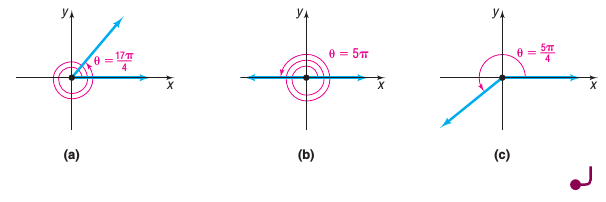
\includegraphics[width=11cm,keepaspectratio=true]{./trig/sull0628.png}
		% sull0628.png: 0x0 pixel, 300dpi, 0.00x0.00 cm, bb=
		\label{fig:0638}
	\end{figure}
	

{}
	\begin{problema}
		Determine el valor exacto de 
		\begin{itemize}
			\item $\sin(405^{o})$
			\item $\cot(390^{o})$
			\item $\sec\left( \dfrac{17\pi}{4} \right)$
		\end{itemize}
		
	\end{problema}
	

{Identidades reciprocas}
	\begin{align}
		\label{sull632}
		\csc(\theta)&= \dfrac{1}{\sin(\theta)}\\
		\sec(\theta)&= \dfrac{1}{\cos(\theta)}\\
		\cot(\theta)&= \dfrac{1}{\tan(\theta)}
	\end{align}

{}
	\begin{problema}
		\label{exmp:6303}
		Dado 
		\begin{align*}
			\sin(\theta)&= \dfrac{\sqrt{5}}{5}\\
			\cos(\theta)&= \dfrac{2\sqrt{5}}{5}
		\end{align*}
		encuentre el valor de las cuatro funciones trigonométricas restantes.
	\end{problema}
	

{}
	\begin{problema}
		\label{exe:6335}
		Dado 
		\begin{align*}
			\sin(\theta)&= -\dfrac{3}{5}\\
			\cos(\theta)&= \dfrac{4}{5}
		\end{align*}
		encuentre el valor de las cuatro funciones trigonométricas restantes.
	\end{problema}
	

{Identidades pitagóricas}
	\begin{align*}
		\sin^{2}\theta+\cos^{2}\theta=1
	\end{align*} 
	\begin{align*}
		\tan^{2}\theta + 1 = \sec^{2}\theta
	\end{align*} 
	\begin{align*}
		\cot^{2}\theta + 1 =\csc^{2}\theta
	\end{align*}


	La función coseno es par:
	$$ \cos(-x)=\cos(x) $$
	mientras que la función seno es impar:
	$$ \sin(-x)=-\sin(x) .$$

{}
	\begin{problema}
		\label{exmp:6304}
		Encuentre el valor exacto de cada expresión \emph{sin usar calculadora}:
		\begin{itemize}
			\item $\tan(20^{o})-\dfrac{\sin(20^{o})}{\cos(20^{o})}$ 
			\item $\sin^{2}\dfrac{\pi}{12}+\dfrac{1}{\sec^{2}\dfrac{\pi}{12}}$
		\end{itemize}
		
	\end{problema}
	

{}
	\begin{problema}
		Encuentre el valor exacto de cada expresión \emph{sin usar la calculadora}:
		\begin{itemize}
			\item $\sin(80^{o})\csc(80^{o})$
			\item $\cos(400^{o})\sec(40^{o})$
			\item $\dfrac{\sin(-20^{o})}{\cos(380^{o})}+\tan(200^{o})$
		\end{itemize}
		
	\end{problema}
	


	\begin{problema}
		\label{exmp:sull6305}
		Dado que $\sin\theta=\frac{1}{3}$ y $\cos\theta$, encuentre el valor exacto de cada una de las restantes cinco funciones trigonométricas.
	\end{problema}
	

{}
	\begin{figure}
		\centering
		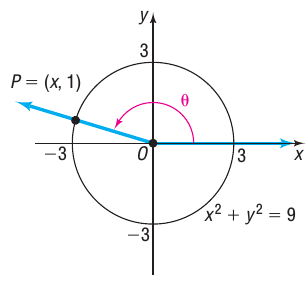
\includegraphics[height=8cm]{./trig/sull0641.png}
		% sull0641.png: 0x0 pixel, 300dpi, 0.00x0.00 cm, bb=
		\label{fig:0641}
	\end{figure}
	

{}
	

{}
	\begin{problema}
		Dado que $\tan\theta=\dfrac{1}{2}$ y $\sin\theta<0$, encuentre el valor exacto de cada una de las restantes cinco funciones trigonométricas en $\theta$.
	\end{problema}
	

{}
	\begin{figure}
		\centering
		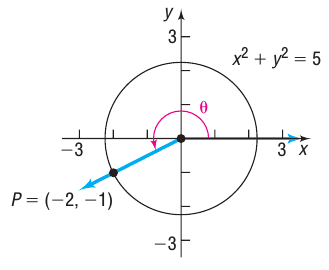
\includegraphics[height=8cm]{./trig/sull0642.png}
		% sull0641.png: 0x0 pixel, 300dpi, 0.00x0.00 cm, bb=
		\label{fig:0642}
	\end{figure}
	

{}
	\begin{problema}
		Encuentre el valor de cada una de las restantes funciones trigonométricas en $\theta$ conociendo que $\sin\theta=\dfrac{12}{13}$ y $\theta$ se encuentra en el segundo cuadrante.
	\end{problema}
	

{Paridad e imparidad}
	Por un lado, una función $f(\theta)$ es par si $f(-\theta)=f(\theta).$  Por otro lado, función $f(\theta)$ si $f(-\theta)=-f(\theta).$

{}
	\begin{figure}
		\centering
		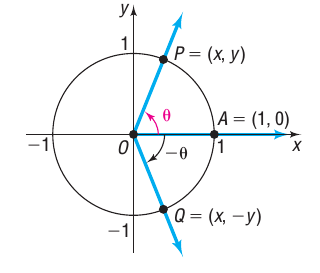
\includegraphics[height=8cm,keepaspectratio=true]{./trig/sull0443.png}
		% sull0443.png: 0x0 pixel, 300dpi, 0.00x0.00 cm, bb=
		\label{fig:0643}
	\end{figure}
	


	\begin{proposicion}
		La función $\cos$ es par, pero la función $\sin$ es par. 
	\end{proposicion}
	

{}
	\begin{problema}
		Determine si las funciones trigonométricas restantes son pares o impares.
	\end{problema}
	

{}
	\begin{problema}
		\label{exmp:0607}
		Encuentre el valor exacto de 
		\begin{itemize}
			\item $\sin(-45^{o})$ 
			\item $\cos(-\pi)$ 
			\item $\cot\left( -\dfrac{3\pi}{2} \right)$ 
			\item $\tan\left( -\dfrac{37\pi}{4} \right)$
		\end{itemize}
		
	\end{problema}
	

{}
	\begin{problema}
		\begin{itemize}
			\item $\sin(-60^{o})$
			\item $\csc(-30^{o})$
			\item $\cos\left( -\dfrac{\pi}{4} \right)$
			\item $\sec(-\pi)$
		\end{itemize}
		
	\end{problema}


\section{Suma y diferencias de ángulos}

{Suma y diferencias para el coseno}
	\begin{align*}
		\cos(s+t) &= \cos(s)\cos(t)-\sin(s)\sin(t) \\  
		\cos(s-t) &= \cos(s)\cos(t)+\sin(s)\sin(t)
	\end{align*}



	\begin{problema} Demuestre las siguientes identidades
		\begin{align*}
			\cos\left(\dfrac{\pi}{2}-t\right) &= \sin(t) \\
			\sin\left(\dfrac{\pi}{2}-t\right) &= \cos(t) 
		\end{align*}
	\end{problema}


{Suma y diferencias para el coseno}
	\begin{align*}
		\sin(s+t) &= \sin(s)\cos(t)+\cos(s)\sin(t) \\  
		\sin(s-t) &= \sin(s)\cos(t)-\cos(s)\sin(t)
	\end{align*}



	\begin{problema}
		Establezca la siguiente identidad
		\begin{align*}
			\dfrac{\cos\left(s-t\right)}{\sin(s)\sin(t)} 
			& = \cot(s)\cot(t)+1
		\end{align*}
	\end{problema}
	



	\begin{problema}
		Demuestre las siguientes identidades
		\begin{enumerate}
			\item $$ \tan(s+t)=\dfrac{\tan s + \tan t}{1- \tan s \tan t} $$ 
			\item $$ \tan(s-t)=\dfrac{\tan s - \tan t}{1+ \tan s \tan t} $$ 
			\item $$ \tan(s+\pi) = \tan(s) $$ 
			\item $$ \tan\left(s+\dfrac{\pi}{2}\right) = -\cot(s) $$
		\end{enumerate}
	\end{problema}



	\begin{problema}
		Demuestre las siguientes identidades
		\begin{enumerate}
			\item $$\sin\left(\dfrac{\pi}{2}+t\right) = \cos t$$
			\item $$\dfrac{\sin\left(s+t\right)}{\sin(s)\cos(t)} = 1+\cot(s)\tan(t)$$
		\end{enumerate}
	\end{problema}

